\documentclass[fleqn, a4paper, 11pt, oneside]{amsart}
\usepackage{exsheets}
\usepackage{amsmath, amssymb, amsthm} %standard AMS packages
\usepackage{marginnote} %marginnotes
\usepackage{gensymb} %miscellaneous symbols
\usepackage{commath} %differential symbols
\usepackage{xcolor} %colours
\usepackage{cancel} %cancelling terms
\usepackage[free-standing-units, space-before-unit]{siunitx} %formatting units
\usepackage{tikz, pgfplots} %diagrams
	\usetikzlibrary{calc, hobby, patterns, intersections, decorations.markings}
\usepackage{graphicx} %inserting graphics
\usepackage{hyperref} %hyperlinks
\usepackage{datetime} %date and time
\usepackage{enumerate,enumitem} %numbered lists
\usepackage{float} %inserting floats
\usepackage{circuitikz}[american voltages, american currents] %circuit diagrams
\usepackage{booktabs}
\usepackage{csvsimple}

\newcommand\numberthis{\addtocounter{equation}{1}\tag{\theequation}} %adds numbers to specific equations in non-numbered list of equations

\theoremstyle{definition}
\newtheorem{example}{Example}
\newtheorem{definition}{Definition}

\theoremstyle{theorem}
\newtheorem{theorem}{Theorem}

\makeatletter
\@addtoreset{section}{part} %resets section numbers in new part
\makeatother

\SetupExSheets{solution/print = true}

%opening
\title
[
	Electronic Devices : Assignment 1
]
{
	Electronic Devices\\
	Assignment 1
}
\author
{
	Aakash Jog\\
	ID : 989323563
}
\date{\formatdate{10}{3}{2016}}

\begin{document}

\maketitle
%\setlength{\mathindent}{0pt}

\begin{question}
	\begin{enumerate}
		\item
			Plot the Fermi function at room temperature for $E_f = 1 \electronvolt$.
			Plot over the energy range $0 \electronvolt - 1.6 \electronvolt$.
			Calculate data points every $0.2 \electronvolt$.
			Attach a table of calculated values along with your plot.
		\item
			Show that the probability of an occupied state $\Delta E$ above $E_f$ is equal to the probability of an empty state $\Delta E$ below $E_F$, i.e.
			\begin{align*}
				f(E_F + \Delta E) & = 1 - f(E_F - \Delta E)
			\end{align*}
	\end{enumerate}
\end{question}

\begin{solution}
	\begin{enumerate}[leftmargin=*]
		\item
			~\\
			\begin{figure}[H]
				\centering
				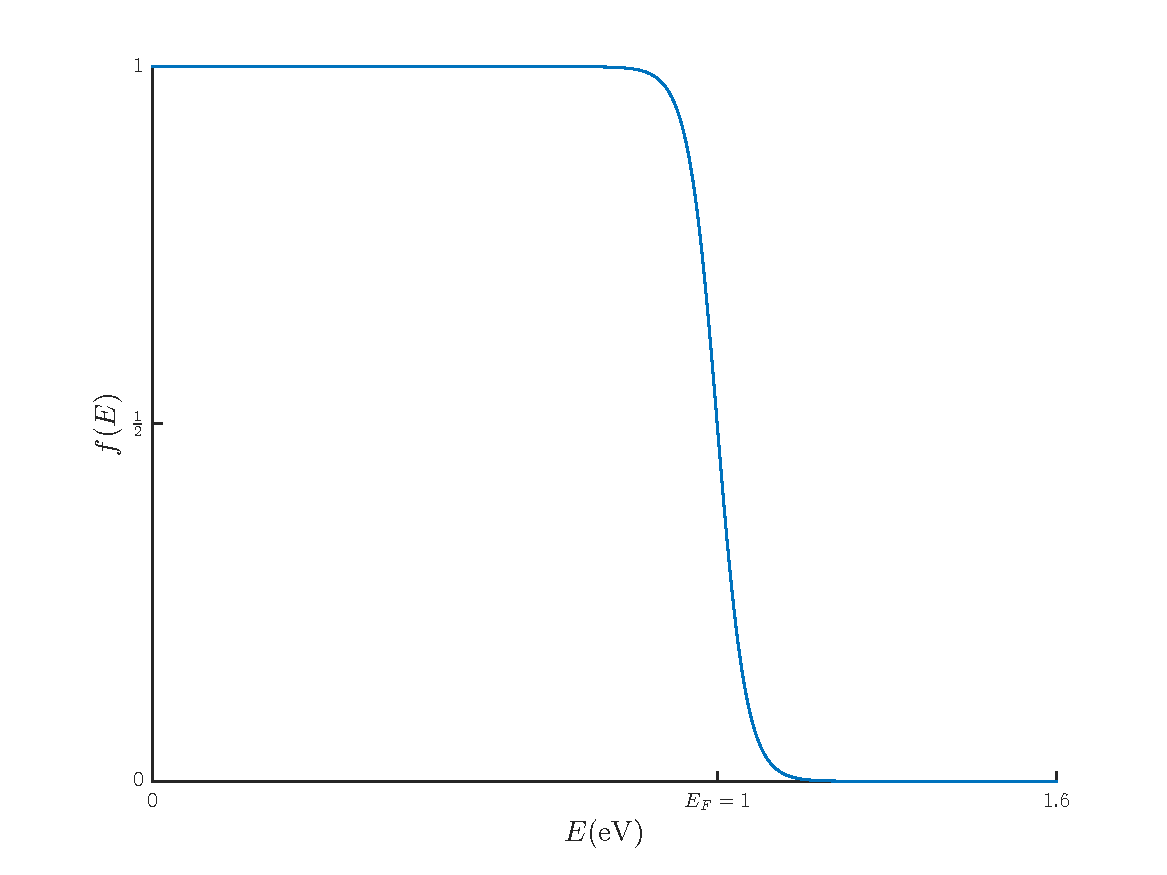
\includegraphics[width = 0.8\textwidth]{./fermi_function.pdf}
			\end{figure}
			\begin{table}[H]
				\centering
				\begin{tabular}{l l}
					\toprule
					$E (\electronvolt)$ & $f(E)$                             \\
					\midrule
					$0$                 & $1$                                \\
					$0.2$               & $0.999999999999964$                \\
					$0.4$               & $0.999999999916739$                \\
					$0.6$               & $0.999999809324428$                \\
					$0.8$               & $0.99956352640943$                 \\
					$1$                 & $0.5$                              \\
					$1.2$               & $0.000436473590570019$             \\
					$1.4$               & $1.90675572317553 \times 10^{-7}$  \\
					$1.6$               & $8.32612088642445 \times 10^{-11}$ \\
					\bottomrule
				\end{tabular}
			\end{table}
		\item
			\begin{align*}
				f(E)                         & = \frac{1}{1 + e^{\frac{E - E_F}{k T}}}                         \\
				\therefore f(E_F + \Delta E) & = \frac{1}{1 + e^{\frac{E_F + \Delta E - E_F}{k T}}}            \\
                                                             & = \frac{1}{1 + e^{\frac{\Delta E}{k T}}}                        \\
				\therefore f(E_F - \Delta E) & = \frac{1}{1 + e^{\frac{E_F - \Delta E - E_F}{k T}}}            \\
                                                             & = \frac{1}{1 + e^{-\frac{\Delta E}{k T}}}                       \\
                                                             & = \frac{e^{\frac{\Delta E}{k T}}}{e^{\frac{\Delta E}{k T}} + 1} \\
                                                             & = 1 - \frac{1}{e^{\frac{\Delta E}{k T}} + 1}                    \\
                                                             & = 1 - f(E_F + \Delta E)
			\end{align*}
	\end{enumerate}
\end{solution}

\begin{question}
	A N-type semiconductor has the following properties.
	\begin{enumerate}
		\item $E_{\text{gap}} = 1.1 \electronvolt$.
		\item $N_C = N_V$.
		\item $N_D = 10^{15} \si{\per\centi\metre\cubed}$.
		\item $E_D = E_C - 0.2 \electronvolt$.
	\end{enumerate}
	Given that $E_f$ is $0.25 \electronvolt$ below $E_C$, calculate $n_i$, and the concentration of the electrons and holes in the semiconductor at $300 \kelvin$.
\end{question}

\begin{solution}
	\begin{align*}
		n                  & = n_i e^{\frac{E_F - E_i}{k T}}             \\
		\therefore N_D     & = n_i e^{\frac{E_F - E_i}{k T}}             \\
		\therefore 10^{15} & = n_i e^{\frac{0.3}{2585.1 \times 10^{-5}}} \\
		\therefore 10^{15} & = n_i e^{11.605}                            \\
		\therefore n_i     & = \frac{10^{15}}{e^{11.605}}                \\
                                   & = 9.12 \times 10^9
	\end{align*}
	Therefore,
	\begin{align*}
		p & = \frac{{n_i}^2}{n}                      \\
                  & = \frac{83.1744 \times 10^{18}}{10^{15}} \\
                  & = 83.1744 10^3
	\end{align*}
\end{solution}

\begin{question}
	A semiconductor has an intrinsic carrier concentration of $10^{10} \si{\per\centi\metre\cubed}$ at $300 \kelvin$, and its conduction and valence band effective densities of states are equal to $10^{19} \si{\per\centi\metre\cubed}$, i.e., $N_C = N_V = 10^{19} \si{\per\centi\metre\cubed}$.
	\begin{enumerate}
		\item
			What is the band gap $E_{\text{gap}}$?
		\item
			If the semiconductor is doped with $N_D = 10^{16} \si{\per\centi\metre\cubed}$, what are the equilibrium electron and hole concentrations at $300 \kelvin$?
		\item
			If the same piece of semiconductor, already having $N_D = 10^{16} \si{\per\centi\metre\cubed}$, is now also doped with acceptors with $N_A = 2 \times 10^{16} \si{\per\centi\metre\cubed}$, what are the new equilibrium electron and hole concentrations at $300 \kelvin$?
			What is the Fermi level position with respect to the intrinsic Fermi level, i.e., what is $E_f - E_i$?
	\end{enumerate}
\end{question}

\begin{solution}
	\begin{enumerate}[leftmargin=*]
		\item
			\begin{align*}
				n_i                                   & = \sqrt{N_C N_V} e^{-\frac{E_{\text{gap}}}{k T}}                  \\
				\therefore \frac{n_i}{\sqrt{N_C N_V}} & = e^{-\frac{E_{\text{gap}}}{k T}}                                 \\
				\therefore E_{\text{gap}}             & = -k T \ln\left( \frac{n_i}{\sqrt{N_C N_V}} \right)               \\
                                                                      & = -(8.617) (300) \ln\left( \frac{10^{10}}{10^{19}} \right)        \\
                                                                      & = -\left( 2585.1 \times 10^{-5} \right) \ln\left( 10^{-9} \right) \\
                                                                      & = -\left( 2585.1 \times 10^{-5} \right) (-20.723)                 \\
                                                                      & = 53571.0273 \times 10^{-5}                                       \\
                                                                      & = 0.53571 \electronvolt
			\end{align*}
		\item
			\begin{align*}
				n & = N_D                                 \\
                                  & = 10^{16} \si{\per\centi\metre\cubed} \\
				p & = \frac{{n_i}^2}{n}                   \\
                                  & = \frac{10^{20}}{10^{16}}             \\
                                  & = 10^4 \si{\per\centi\metre\cubed}
			\end{align*}
		\item
			\begin{align*}
				p & = N_A - N_D                           \\
                                  & = 10^{16} \si{\per\centi\metre\cubed} \\
				n & = \frac{{n_i}^2}{p}                   \\
                                  & = \frac{10^{20}}{10^{16}}             \\
                                  & = 10^4 \si{\per\centi\metre\cubed}
			\end{align*}
			Therefore,
			\begin{align*}
				n                                    & = n_i e^{\frac{E_F - E_i}{k T}}                                           \\
				\therefore 10^{4}                    & = 10^{10} e^{\frac{E_F - E_i}{\left( 8.617 \times 10^{-5} \right) (300)}} \\
				\therefore 10^{-6}                   & = e^{\frac{E_F - E_i}{2585.1 \times 10^{-5}}}                             \\
				\therefore \ln\left( 10^{-6} \right) & = \frac{E_F - E_i}{2585.1 \times 10^{-5}}                                 \\
				\therefore E_F - E_i                 & = (-13.8155) \left( 2585.1 \times 10^{-5} \right)                         \\
                                                                     & = -0.3571444905
			\end{align*}
	\end{enumerate}
\end{solution}

\end{document}
